\documentclass[tikz]{standalone} 
\usepackage{spath}
\usepackage{tikz}
\usetikzlibrary{calc}
\usetikzlibrary{fadings}

\begin{document}

% Source: LaTeX-Community.org 
%         <http://www.latex-community.org/viewtopic.php?f=4&t=2111>
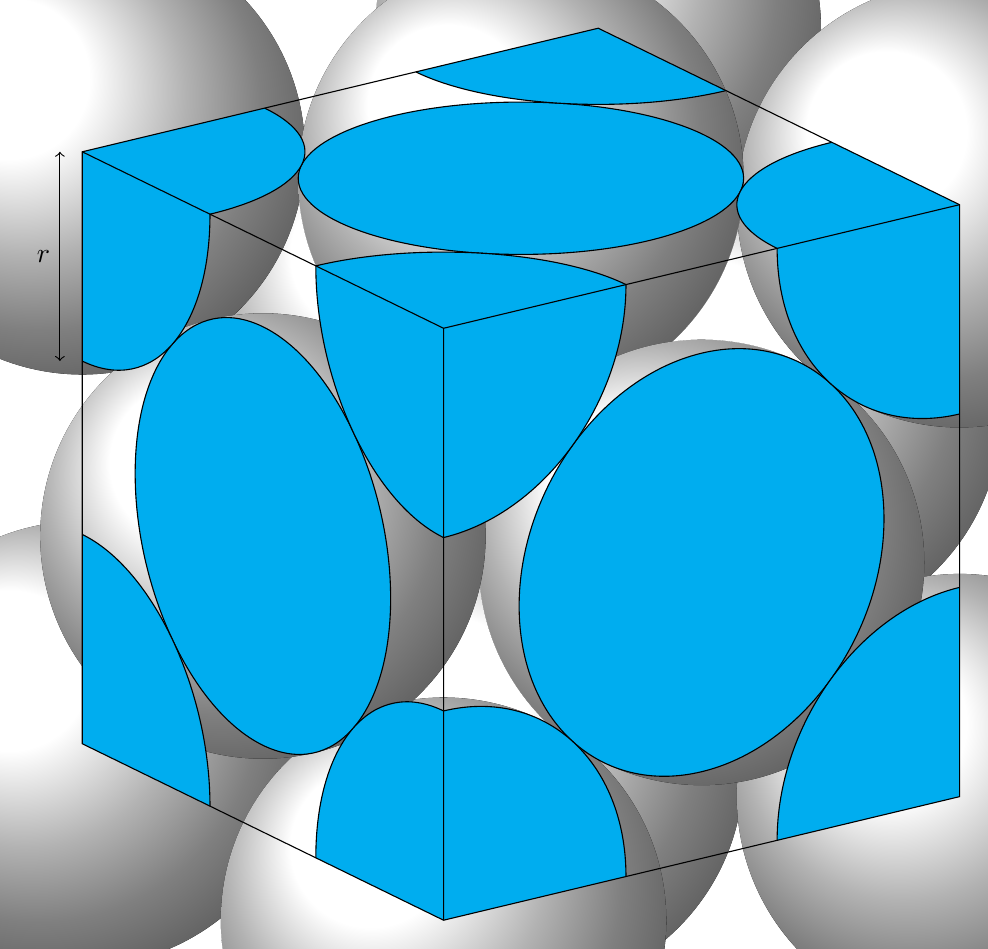
\begin{tikzpicture}
\newcommand\pgfmathsinandcos[3]{%
  \pgfmathsetmacro#1{sin(#3)}%
  \pgfmathsetmacro#2{cos(#3)}%
}
\newcommand\LongitudePlane[3][current plane]{%
  \pgfmathsinandcos\sinEl\cosEl{#2} % elevation
  \pgfmathsinandcos\sint\cost{#3} % azimuth
  \tikzset{#1/.style={cm={\cost,\sint*\sinEl,0,\cosEl,(0,0)}}}
}
\newcommand\LatitudePlane[3][current plane]{%
  \pgfmathsinandcos\sinEl\cosEl{#2} % elevation
  \pgfmathsinandcos\sint\cost{#3} % latitude
  \pgfmathsetmacro\yshift{\cosEl*\sint}
  \tikzset{#1/.style={cm={\cost,0,0,\cost*\sinEl,(0,\yshift)}}}
}

%\newcommand\DrawLongitudeCircle[2][4]{
%  \LongitudePlane{\angEl}{#2}
%%  \tikzset{current plane/.prefix style={scale=#1}}
%   % angle of "visibility"
%  \pgfmathsetmacro\angVis{atan(sin(#2)*cos(\angEl)/sin(\angEl))}
%  \draw[current plane, blue] (\angVis:\R) arc (\angVis:\angVis+180:\R);
%  \draw[current plane, blue] (\angVis-180:\R) arc (\angVis-180:\angVis:\R);
%}

%\newcommand\DrawLatitudeCircle[2][5]{
%  \LatitudePlane{\angEl}{#2}
%%  \tikzset{current plane/.prefix style={scale=#1}}
%%  \pgfmathsetmacro\sinVis{sin(#2)/cos(#2)*sin(\angEl)/cos(\angEl)}
%%  % angle of "visibility"
%%  \pgfmathsetmacro\angVis{asin(min(1,max(\sinVis,-1)))}
%  \draw[current plane, red] (\angVis:\R) arc (\angVis:-\angVis-180:\R);
%  \draw[current plane, red] (180-\angVis:\R) arc (180-\angVis:\angVis:\R);
%}

\newcommand\ClipLongitudeCircle[2]{
    \LongitudePlane{\angEl}{#1}
    \pgfmathsetmacro\angVis{atan(sin(#1)*cos(\angEl)/sin(\angEl))}
    \path[save path=\tmppath, current plane] (\angVis:\R) arc (\angVis:\angVis+180:\R); % current plane transformation
    \pgfoonew\patha=new spath(\tmppath)
    \pgfmathsetmacro\angVis{-atan(sin(\angEl)*cos(#1)/sin(#1))}
    \path[save path=\tmppath] (-90+\angVis:\R) arc (-90+\angVis:#2 180-90+\angVis:\R); % no coordinate transform (no current plane)
    \pgfoonew\pathb=new spath(\tmppath)
    \patha.concatenate with lineto(,\pathb)
    \patha.close()
    \patha.use path with tikz(clip)
%   \patha.use path with tikz(fill=magenta, opacity=.2)
%   \patha.use path with tikz(draw=magenta, very thick)
}

\newcommand\ClipLatitudeCircle[2]{
    \LatitudePlane{\angEl}{#1}
    \path[save path=\tmppath,current plane] (-180:\R) arc (-180:0:\R);
    \pgfoonew\patha=new spath(\tmppath)
    \path[save path=\tmppath] (0:\R) arc (0:#2 180:\R);
    \pgfoonew\pathb=new spath(\tmppath)
    \patha.concatenate with lineto(,\pathb)
    \patha.close()
    \patha.use path with tikz(clip)
%   \patha.use path with tikz(fill=cyan, opacity=.2)
%   \patha.use path with tikz(draw=cyan, very thick)
}

\newcommand\ClippedEightSphere[4]{
\begin{scope}[transform canvas={shift=(#4)}]
    \ClipLongitudeCircle{45-\angPh}{#1}
    \ClipLongitudeCircle{135-\angPh}{#2}
    \ClipLatitudeCircle{0}{#3}
    \fill[ball color=white] (0,0) circle (\R);
\end{scope}}

\newcommand\ClippedLatitudeSphere[3]{
\begin{scope}[transform canvas={shift=(#1)}]
    \LatitudePlane{\angEl}{#2}
    \ClipLatitudeCircle{0}{#3}
    \fill[ball color=white] (0,0) circle [radius=\R];
\end{scope}}

\newcommand\ClippedLongitudeSphere[3]{
\begin{scope}[transform canvas={shift=(#1)}]
    \LongitudePlane{\angEl}{#2}
    \ClipLongitudeCircle{#2}{#3}
    \fill[ball color=white] (0,0) circle [radius=\R];
\end{scope}}

\newcommand\DrawLongitudeArc[4]{
    \LongitudePlane{\angEl}{#2}
    \begin{scope}[current plane, transform canvas={shift=(#1)}]
    \fill [cyan] (0,0) -- ++(#3:\R) arc [start angle=#3, delta angle=#4, radius=\R] -- cycle;
    \draw ++(#3:\R) arc [start angle=#3, delta angle=#4, radius=\R];
    \end{scope}}

\newcommand\DrawLatitudeArc[4]{
    \LatitudePlane{\angEl}{#2}
    \begin{scope}[current plane, transform canvas={shift=(#1)}]
    \fill [cyan] (0,0) -- ++(#3:\R) arc [start angle=#3, delta angle=#4, radius=\R] -- cycle;
    \draw ++(#3:\R) arc [start angle=#3, delta angle=#4, radius=\R];
    \end{scope}}



    \def\D{8} % cubic side length
%   \pgfmathsetmacro\R{\D/2} % sphere radius
    \pgfmathsetmacro\R{sqrt(2)/4*\D} % sphere radius
%   \pgfmathsetmacro\R{sqrt(3)/4*\D} % sphere radius
    \def\angEl{20} % elevation angle in interval [1,89]
    \def\angPh{10} % phase angle in interval [-44,44]
    \pgfmathsetmacro\uofx{cos(-135-\angPh)}
    \pgfmathsetmacro\vofx{sin(-135-\angPh)*sin(\angEl)}
    \pgfmathsetmacro\uofy{cos(-45-\angPh)}
    \pgfmathsetmacro\vofy{sin(-45-\angPh)*sin(\angEl)}
    \pgfmathsetmacro\uofz{0}
    \pgfmathsetmacro\vofz{cos(\angEl)}

    % The coordinates of the cube
    \begin{scope}[x={(\uofx cm,\vofx cm)}, y={(\uofy cm,\vofy cm)}, z={(\uofz cm,\vofz cm)}]
    \coordinate (C1) at (\D,0,0);
    \coordinate (C2) at (\D,0,\D);
    \coordinate (C3) at (0,0,\D);
    \coordinate (C4) at (0,\D,\D);
    \coordinate (C5) at (0,\D,0);
    \coordinate (C6) at (\D,\D,0);
    \coordinate (C7) at (0,0,0);
    \coordinate (C8) at (\D,\D,\D);
%    \foreach \n in {1,2,...,8} \node at (C\n) {C\n};

    \coordinate (C0) at ($(C2)!.5!(C5)$);
    \coordinate (S1) at ($(C2)!.5!(C6)$);
    \coordinate (S2) at ($(C2)!.5!(C4)$);
    \coordinate (S3) at ($(C8)!.5!(C5)$);
    \coordinate (S4) at ($(C6)!.5!(C7)$);
    \coordinate (S5) at ($(C1)!.5!(C3)$);
    \coordinate (S6) at ($(C5)!.5!(C3)$);
    \end{scope}

    % Draw the clipped spheres
    \ClippedEightSphere{+}{-}{+}{C7}
    \ClippedLongitudeSphere{S5}{45-\angPh}{+}
    \ClippedLongitudeSphere{S6}{135-\angPh}{-}
    \ClippedLatitudeSphere{S4}{0}{+}

    \ClippedEightSphere{-}{+}{-}{C8}
    \ClippedEightSphere{+}{-}{-}{C3}
    \ClippedEightSphere{+}{+}{-}{C2}
%   \fill[ball color=white] (C0) circle [radius=\R];
    \ClippedEightSphere{-}{-}{-}{C4}
    \ClippedEightSphere{+}{+}{+}{C1}
    \ClippedEightSphere{-}{-}{+}{C5}
    \ClippedEightSphere{-}{+}{+}{C6}

    % Draw the half spheres
    \ClippedLatitudeSphere{S2}{0}{-}
    \ClippedLongitudeSphere{S3}{45-\angPh}{-}
    \ClippedLongitudeSphere{S1}{135-\angPh}{+}
    \DrawLatitudeArc{S2}{0}{0}{360}
    \DrawLongitudeArc{S1}{135-\angPh}{0}{360}
    \DrawLongitudeArc{S3}{45-\angPh}{0}{360}

    % Draw the Arcs
    \DrawLongitudeArc{C1}{135-\angPh}{90}{90}
    \DrawLongitudeArc{C2}{135-\angPh}{-90}{-90}
    \DrawLongitudeArc{C4}{45-\angPh}{-90}{-90}
    \DrawLongitudeArc{C5}{45-\angPh}{90}{90}
    \DrawLongitudeArc{C6}{135-\angPh}{90}{-90}
    \DrawLongitudeArc{C6}{45-\angPh}{90}{-90}
    \DrawLongitudeArc{C8}{135-\angPh}{-90}{90}
    \DrawLongitudeArc{C8}{45-\angPh}{-90}{90}
    \DrawLatitudeArc{C2}{0}{45-\angPh}{-90}
    \DrawLatitudeArc{C3}{0}{-45-\angPh}{-90}
    \DrawLatitudeArc{C4}{0}{135-\angPh}{90}
    \DrawLatitudeArc{C8}{0}{135-\angPh}{-90}

    % Draw the cube
    \draw (C1)--(C2)--(C3)--(C4)--(C5)--(C6)--cycle;
    \draw (C2)--(C8)--(C6);
    \draw (C8)--(C4);

    % Radius node
    \coordinate (r) at ($(C2) - (\R/10,0)$);
    \LongitudePlane{\angEl}{135-\angPh}
    \draw [<->, current plane] (r) -- node [left] {$r$} +(-90:\R);

\end{tikzpicture}
\end{document}
